% ---
% Capa
% ---
\imprimircapa
% ---

% ---
% Folha de rosto
% (o * indica que haverá a ficha bibliográfica)
% ---
\imprimirfolhaderosto*
% ---

% ---
% Inserir a ficha bibliografica
% ---
% http://ficha.bu.ufsc.br/
\begin{fichacatalografica}
	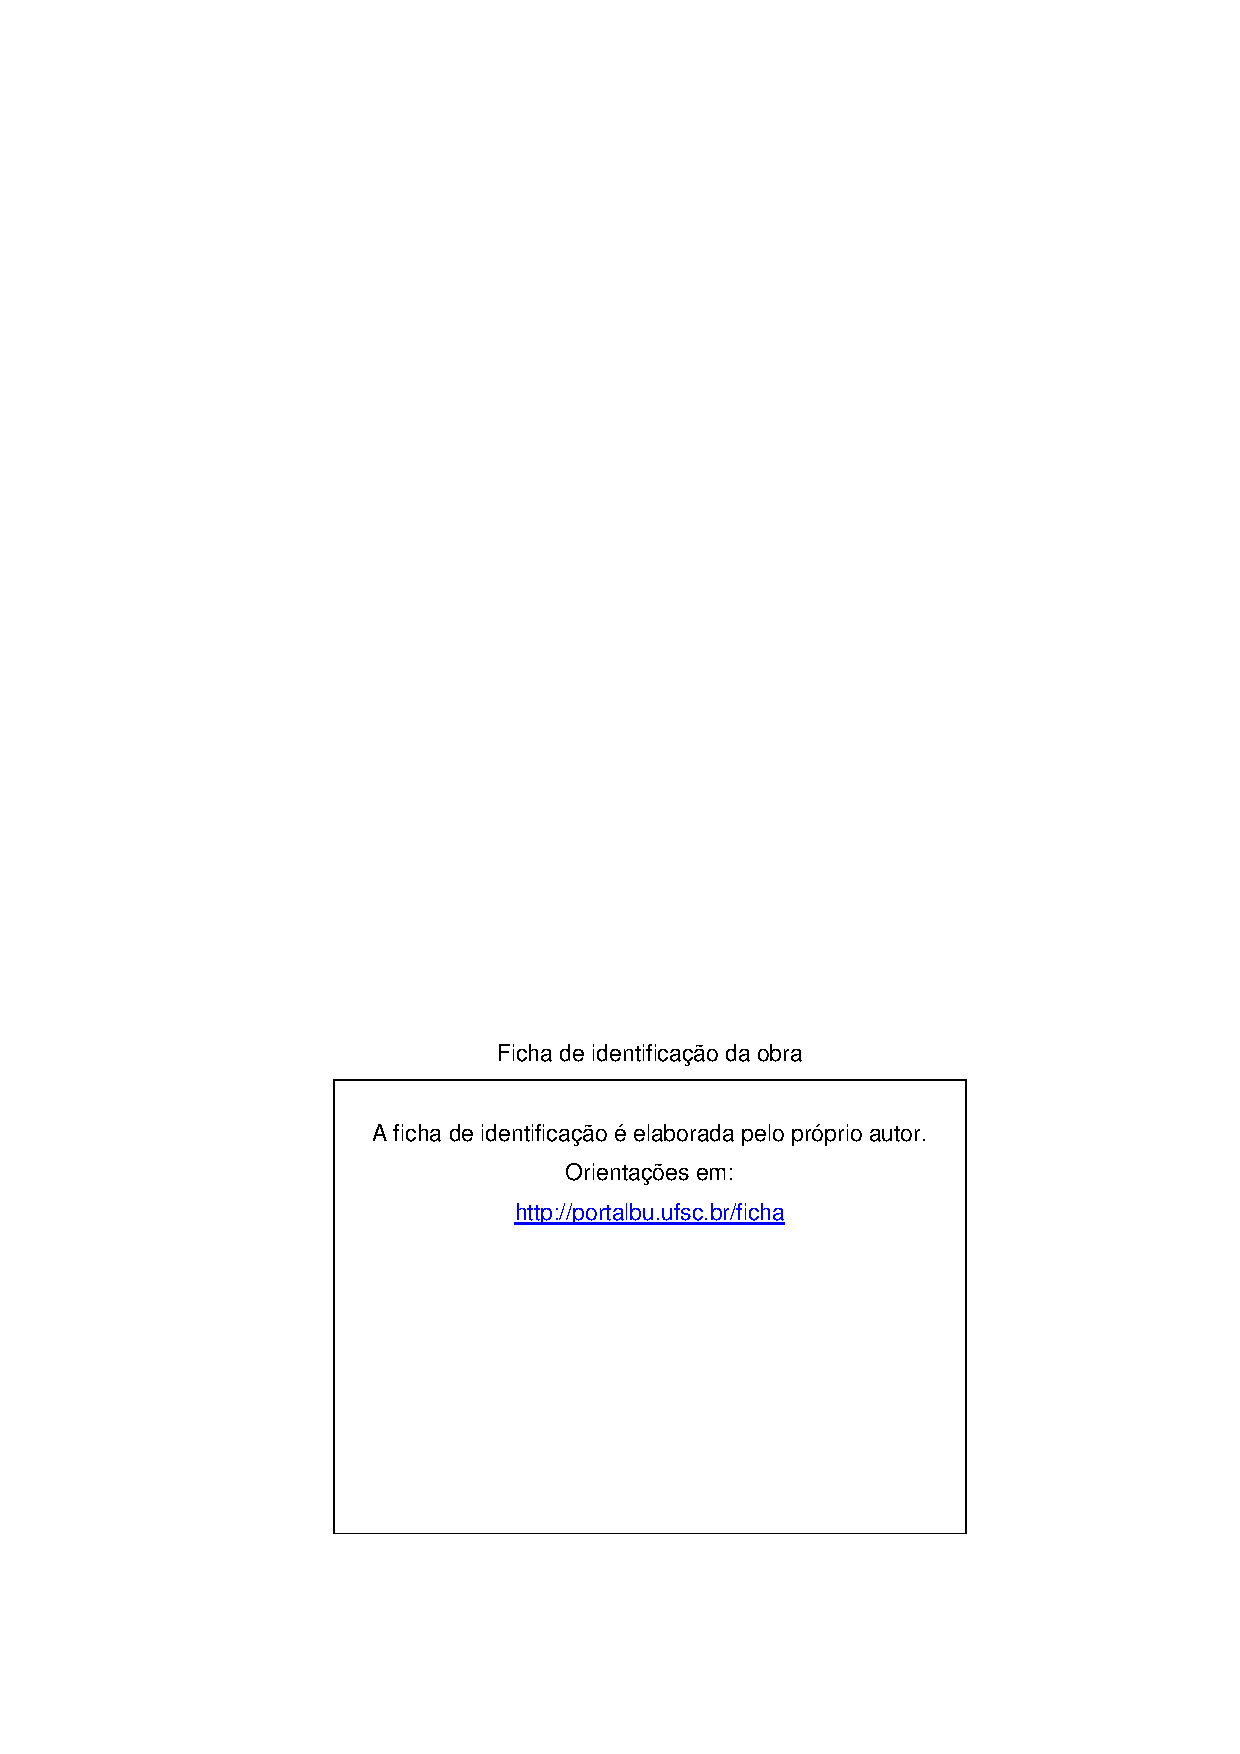
\includepdf{beforetext/Ficha_Catalografica.pdf}
\end{fichacatalografica}
% ---

% ---
% Inserir folha de aprovação
% ---
\begin{folhadeaprovacao}
	\OnehalfSpacing
	\centering
	\imprimirautor\\%
	\vspace*{10pt}		
	\textbf{\imprimirtitulo}%
	\ifnotempty{\imprimirsubtitulo}{:~\imprimirsubtitulo}\\%
	%		\vspace*{31.5pt}%3\baselineskip
	\vspace*{\baselineskip}
	%\begin{minipage}{\textwidth}
	% ~do~\imprimirprograma~do~\imprimircentro~da~\imprimirinstituicao~para~a~obtenção~do~título~de~\imprimirformacao.
	Este~\imprimirtipotrabalho~foi julgado adequado para obtenção do Título de “\imprimirformacao” e aprovado em sua forma final pelo~\imprimirprograma. \\
		\vspace*{\baselineskip}
	\imprimirlocal, \imprimirdata. \\
	\vspace*{2\baselineskip}
	\assinatura{\OnehalfSpacing\imprimircoordenador \\ \imprimircoordenadorRotulo~do Curso}
	\vspace*{2\baselineskip}
	\textbf{Banca Examinadora:} \\
	\vspace*{\baselineskip}
	\assinatura{\OnehalfSpacing\imprimirorientador \\ \imprimirorientadorRotulo}
	%\end{minipage}%
	\vspace*{\baselineskip}
	\assinatura{Prof.(a) xxxx, Dr(a).\\
	Avaliador(a) \\
	Instituição xxxx}

	\vspace*{\baselineskip}
	\assinatura{Prof.(a) xxxx, Dr(a).\\
	Avaliador(a) \\
	Instituição xxxx}


\end{folhadeaprovacao}
% ---

% ---
% Dedicatória
% ---
\begin{dedicatoria}
	\vspace*{\fill}
	\noindent
	\begin{adjustwidth*}{}{5.5cm}     
		Dedico o presente trabalho à minha mãe, que meu fazer ciência seja tão legal aos seus olhos quanto nos filmes que assistimos juntos.
		
	\end{adjustwidth*}
\end{dedicatoria}
% ---

% ---
% Agradecimentos
% ---
\begin{agradecimentos}
	Inserir os agradecimentos aos colaboradores à execução do trabalho. 
	
	Xxxxxxxxxxxxxxxxxxxxxxxxxxxxxxxxxxxxxxxxxxxxxxxxxxxxxxxxxxxxxxxxxxxxxx. 
\end{agradecimentos}
% ---

% ---
% Epígrafe
% ---
\begin{epigrafe}
	\vspace*{\fill}
	\begin{flushright}
		\textit{“Acredito que a única coisa 	 mais importante,\\
		 além da disciplina e da criatividade,\\ 
		é ter a coragem de arriscar.”\\
			— Maya Angelou
		}
	\end{flushright}
\end{epigrafe}
% ---

% ---
% RESUMOS
% ---

% resumo em português
\setlength{\absparsep}{18pt} % ajusta o espaçamento dos parágrafos do resumo
\begin{resumo}
	\SingleSpacing
Durante o mês de setembro de 2024, ocorreu sobre todo o estado de Santa Catarina, Brasil diversos fenômenos atmosféricos associados à poluição do ar, como eventos de black rain, quedas bruscas nos índices de qualidade do ar e consequentemente o agravamento de doenças respiratórias na população. Na época, a região oeste do estado não apresentava estações de qualidade do ar ativas, gerando uma lacuna de informações detalhadas sobre os impactos desses fenômenos no território. No presente trabalho é proposto estudo de caso a partir de dados meteorológicos de diferentes reanálises globais com os objetivos de: Identificar os períodos de maior presença de aerossóis na atmosfera (bem como as espécies de poluentes presentes); Investigar o padrão atmosférico que pode ter contribuído para o transporte desses poluentes até o estado de SC; E simular através do modelo de trajetória híbrida HYSPLIT o transporte e dispersão desses aerossóis levando em conta as características da atmosfera, as propriedades físico-químicas dos aerossóis identificados na primeira parte do estudo e a ocorrência de incêndios na floresta amazônica na época. Resultados preliminares indicam que a região oeste do estado foi a mais afetada, reforçando a necessidade de investigações mais detalhadas neste recorte geográfico.
	
	\textbf{Palavras-chave}: Palavra-chave 1. Palavra-chave 2. Palavra-chave 3.
\end{resumo}

% resumo em inglês
\begin{resumo}[Abstract]
	\SingleSpacing
	\begin{otherlanguage*}{english}
		During September 2024, the state of Santa Catarina, Brazil was the stage for several atmospheric phenomena associated with air pollution, such as black rain, sudden drops in air quality indexes and therefore the aggravation of respiratory diseases in the population. At the time, the western region of the state didn’t have active air quality meteorologic stations, which culminated in a lack of detailed information on the impacts of such occurrences in the territory. In the present work it is proposed a case study starting from data made available by different global reanalyses with the following goals: Identifying the periods of highest aerosol occurrence in the atmosphere (as well as the species of pollutants that were registered); Assessing the atmospheric pattern that may have contributed to the transport of these pollutants to the state of SC; And simulating with the HYSPLIT hybrid trajectory model the transport and dispersion of these aerosols taking into account the physical and chemical properties of the pollutants identified in the first part of the study and the occurrence of wildfires in the amazon forest at the time. Preliminary results indicate that the western region was the most affected, reinforcing the need for further detailed investigation in this geographic scope.
		
		
		\textbf{Keywords}: Keyword 1. Keyword 2. Keyword 3.
	\end{otherlanguage*}
\end{resumo}

%% resumo em francês 
%\begin{resumo}[Résumé]
% \begin{otherlanguage*}{french}
%    Il s'agit d'un résumé en français.
% 
%   \textbf{Mots-clés}: latex. abntex. publication de textes.
% \end{otherlanguage*}
%\end{resumo}
%
%% resumo em espanhol
%\begin{resumo}[Resumen]
% \begin{otherlanguage*}{spanish}
%   Este es el resumen en español.
%  
%   \textbf{Palabras clave}: latex. abntex. publicación de textos.
% \end{otherlanguage*}
%\end{resumo}
%% ---

{%hidelinks
	\hypersetup{hidelinks}
	% ---
	% inserir lista de ilustrações
	% ---
	%\pdfbookmark[0]{\listfigurename}{lof}
	%\listoffigures*
	%\cleardoublepage
	% ---
	
	% ---
	% inserir lista de quadros
	% ---
	%\pdfbookmark[0]{\listofquadrosname}{loq}
	%\listofquadros*
	%\cleardoublepage
	% ---
	
	% ---
	% inserir lista de tabelas
	% ---
	%\pdfbookmark[0]{\listtablename}{lot}
	%\listoftables*
	%\cleardoublepage
	% ---
	
	% ---
	% inserir lista de abreviaturas e siglas (devem ser declarados no preambulo)
	% ---
	%\imprimirlistadesiglas
	% ---
	
	% ---
	% inserir lista de símbolos (devem ser declarados no preambulo)
	% ---
	%\imprimirlistadesimbolos
	% ---
	
	% ---
	% inserir o sumario
	% ---
	\pdfbookmark[0]{\contentsname}{toc}
	\tableofcontents*
	\cleardoublepage
	
}%hidelinks
% ---